\documentclass[12pt,a4paper]{article}
\usepackage[utf8]{inputenc}
\usepackage{graphicx}
\usepackage{tikz}
\usetikzlibrary{fit}
\usepackage{lmodern}
\usepackage{sectsty}


\sectionfont{\color{cyan}}

\begin{document}
   \begin{titlepage}
      {\fontfamily{lmss}\selectfont
      	\centering
      	
\includegraphics[width=0.30\textwidth]{logo.png}\par\vspace{1cm}
      	{\LARGE Compiax \par}
      	\vspace{0.25cm}
      	{\huge\bfseries \color{cyan}SplitBill\par}
      	\vspace{1cm}
      	{\Large\textit{by} Brute Force\par}
         \vspace{0.25cm}
         \begin{tikzpicture}
            \node [inner sep=0pt,,outer sep=0pt,clip,rounded corners=0.5cm] (pict) at (0,0) {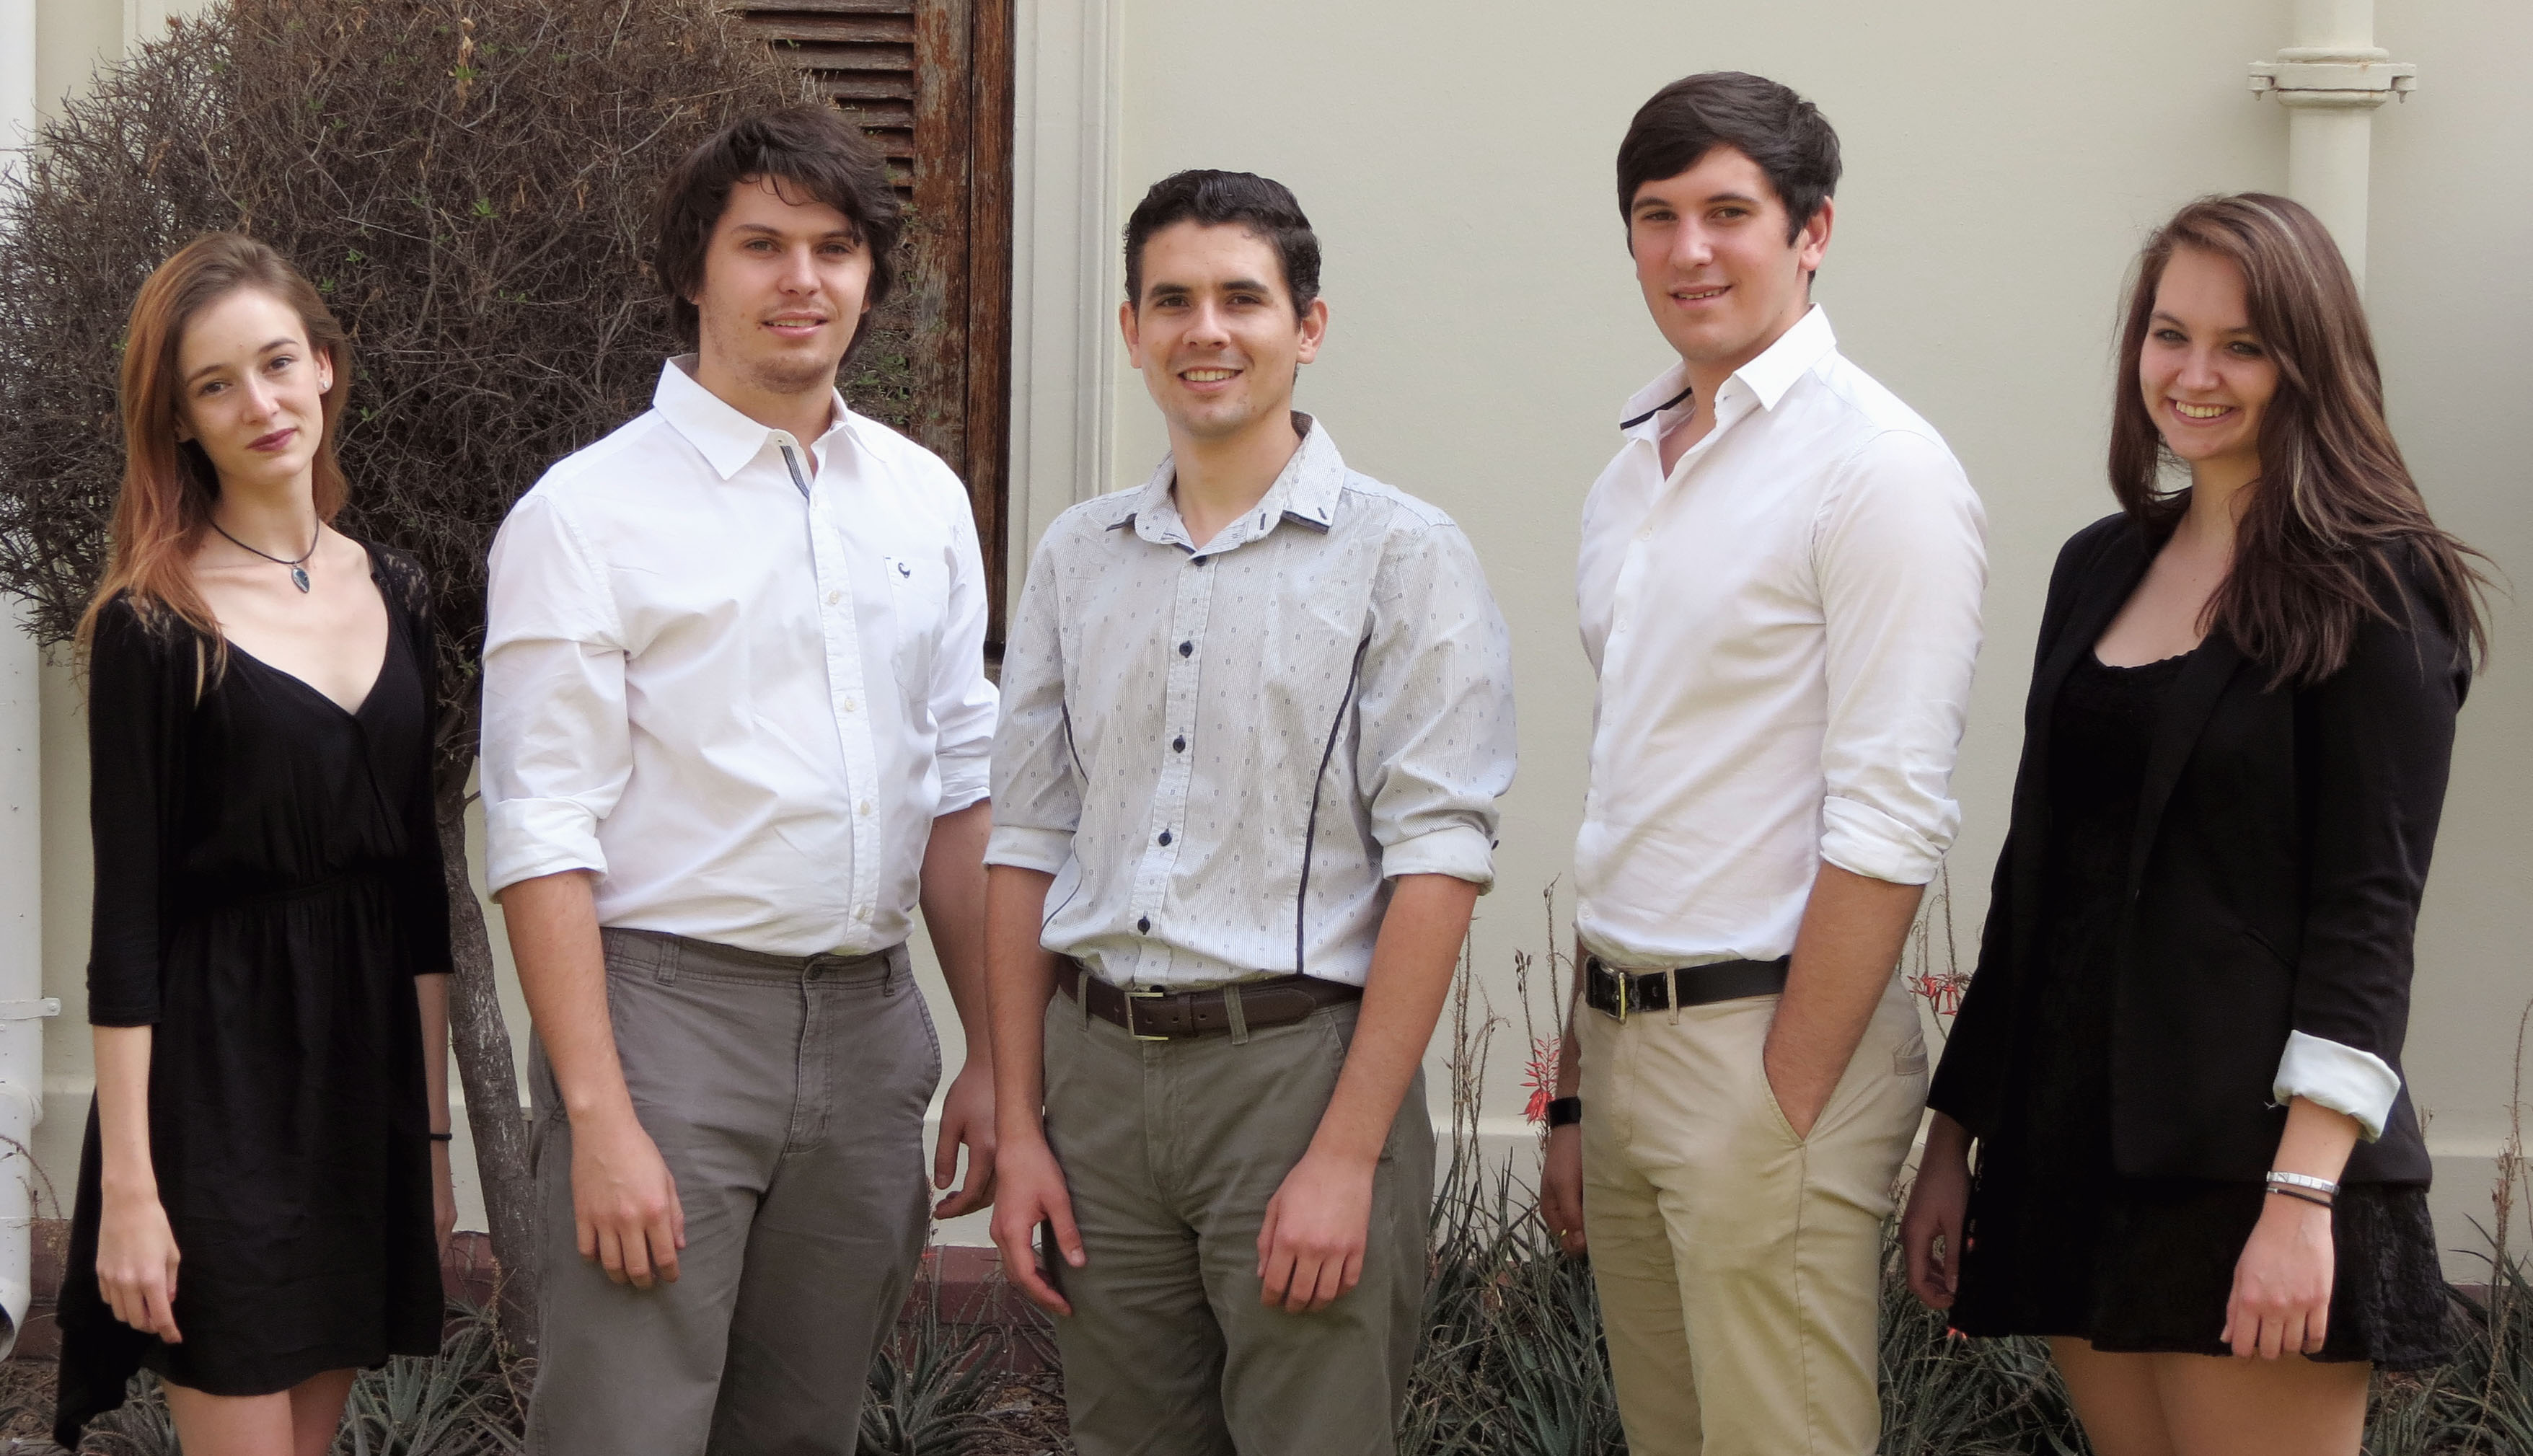
\includegraphics[width=0.9\textwidth]{team.jpg}};
            \node[fit=(pict),rounded corners=.55cm,inner sep=2pt]{};
         \end{tikzpicture}

         \par\vspace{1cm}
         \date{}
         \author{}
         \title{}
         \centering
         \textbf{Authors:}\\
         Mia Gerber\\
         Matthew Perry\\
         Wanrick Willemse\\
         Duart Breedt\\
         Linda Potgieter\\
      }
   \end{titlepage}
   \maketitle
   \tableofcontents
   \newpage

   \section{Introduction}
   The project presented is the development of a mobile application that will manage the division of items on a restaurant receipt among the patrons around the table. We believe this product can be extended to manage
   collective shopping receipts and essentially any receipt that contains items that needs to be split among users. This document serves as our proposal of how to address this issue.

   \section{Project description}
   At the highest level our objective is to create a user friendly app, that is visually appealing and enjoyable to use. The following high level requirements are to be met:
   \begin{itemize}
      \item \textbf{Capture and interpret the receipt}\\
         For this we are considering Tesseract-OCR.\@ Tesseract is an open-source OCR library, sponsored by Google. Mobile libraries exist for both Andriod and iOS.\@ This can be used with no charge.\\
         An alternative would be Google's Mobile Vision API.\@ This however comes with some limitations with regards to daily usage and fees may be incurred with a large user base. For development and testing purposes, this
         should not be a problem.
      \item \textbf{Add users}\\
         One user will be required to take a photo of the receipt. This user will act as the host of the session. By using NFC or QR scan other users will be added to the bill. If a user does not have the app installed, any
         other user will be allowed to add a `guest' whose bill can then be calculated.
      \item \textbf{Provide an interface}\\
         The app interface will be built using AngularJS and Ionic. This will ensure a cross-platform application.
      \item \textbf{Live sync}\\
         For offline sync we are looking into Couchbase lite to handle peer to peer replication. Couchbase is fully integratable into the MEAN stack essentially replacing MongoDB.\@ Authentication and connection information can
         then be tranferred using NFC or a QR barcode.\\
         Using MongoDB may require internet access when syncing in real time.\\
         Bluetooth is also very limited in the amount of devices it allows and currently compatibility between Android and iOS bluetooth devices is questionable at best.
      \item \textbf{Learn}\\
         Adding functionality for learning new receipt formats will be done by extending the user interface and further utilizing the OCR component. Input from the user will divide the image into the appropriate fields and the
         format can be stored in JSON format.
      \item \textbf{App and server}\\
         Server functionality will be useful for centralizing the formats of receipts, and result in a smaller app size if the format of a receipt is fetched from an online database. As a team we agree that the pros and cons of
         using a server must be carefully considered. We intend to make the application as cost-effective as possible.
   \end{itemize}
   Basic planned functionality is as follows. A user takes a picture of the receipt and this is processed and represented on the user interface. The user is then given the option to invite other to join this receipt. Checkboxes
   next to items allow users to claim items and a subtotal is generated for each user. Each user is then given the opportunity to add a tip. On each device the total for the receipt is displayed, as well as the subtotal for the
   specific user and the total that the group's contributions amount to.

   \section{Development Methodologies}
   \subsection{Interaction between development team and client}
   Primarily we believe our client to be the expert and we aim to meet the needs stipulated to us, in an accurate and timely manner. Not only to build a good quality product, but a useful one. With SplitBill we will rely on our
   collective knowledge and experience, the client's and our team's, to create a useful receipt sharing solution. A detailed expectation breakdown will be discussed if we are given this opportunity.

   Our team will strictly adhere to Agile Development Principles. The client will primarily be involved in testing and the feedback will serve as reference for future releases. It is important to us that the scope of the product
   is discussed and agreed upon by both the client, and our team. We are aware that requirements may change, but to ensure that a quality, useful product results from the available time-frame, we prefer to have an agreed upon
   feature list to direct our course.

   \subsection{Interaction between members of development team}
   Our team will apply SCRUM methodologies in order to structure how teamwork will occur for this project, this is a faster, more intensely iterative approach to controlling workflow.

   We are using Slack and ZenHub (in conjunction with Github) to ensure that team members are aware of each other even when we are not physically together and are alerted when work is either available or completed.
	Meetings will be held once a week regardless of the state of the project. Each meeting will require that each team member give a small summary of work done that week, enforcing accountability.
   Working in weekly `sprints' also optimizes predictability and minimizes risk (if something does go wrong it is only a week's worth of work lost, not a whole month.)

   As a team we are going to be adhering to a practice called `pair-programming' which is essentially two or more people working on the same piece of code or feature in order to maximize the chances of bugs
   being discovered and minimize the time required to get a feature ready for production.

   \section{Our Team}
   Team details here:
   Brute Force is a ragtag team of stalwart friends, off on a whirlwind big city adventure.
\end{document}
